\section{Performance Analysis}
\label{sec:4}
\noindent The system in Fig.~\ref{fig:2} is simulated in \textbf{MATLAB} with 
$K = 64$ subcarriers, $L = 1$ multicarrier symbol per packet, and $\Mtot = 4K$. 
The total available SU TX transmit power is $\ptot = K$. 
Assuming the thermal noises at both the PU RX and SU RX arise from the same type 
of front-end amplifiers, we choose $\sigma_{\mathrm{P},\mathrm{W}}^2 = \sigma_{\mathrm{S},\mathrm{W}}^2$. 
Similarly, as both PU and SU coexist in the same band (e.g., an industrial, scientific and medical band), 
we assume the TPI profiles $\sigma_{\mathrm{P},I,k}^2 = \sigma_{\mathrm{S},I,k}^2$ and 
the average TPI power 
$\frac{1}{K} \sum_{k \in \Omega_{0,K}} \sigma_{\mathrm{S},I,k}^2 = \sigma_{\mathrm{S},\mathrm{W}}^2$. 
The interference temperature is chosen as 
$i_{\mathrm{temp}} = \beta \, \pp \, \sigma_{\mathrm{P}}^2 \, \sigma_{\mathrm{P},\mathrm{W}}^2$ 
with the allowed interference power relative to the thermal noise interference at the PU RX 
to be $\beta = 5$ and a confidence level $a = 0.9$. 
Furthermore, for simplicity, $\sigma_{\mathrm{SP}}^2 = 1/\sigma_{\mathrm{PS}}^2$ and $\pp = \sigma_{\mathrm{S},\mathrm{W}}^2$. 

\begin{figure}[htbp]
\centering
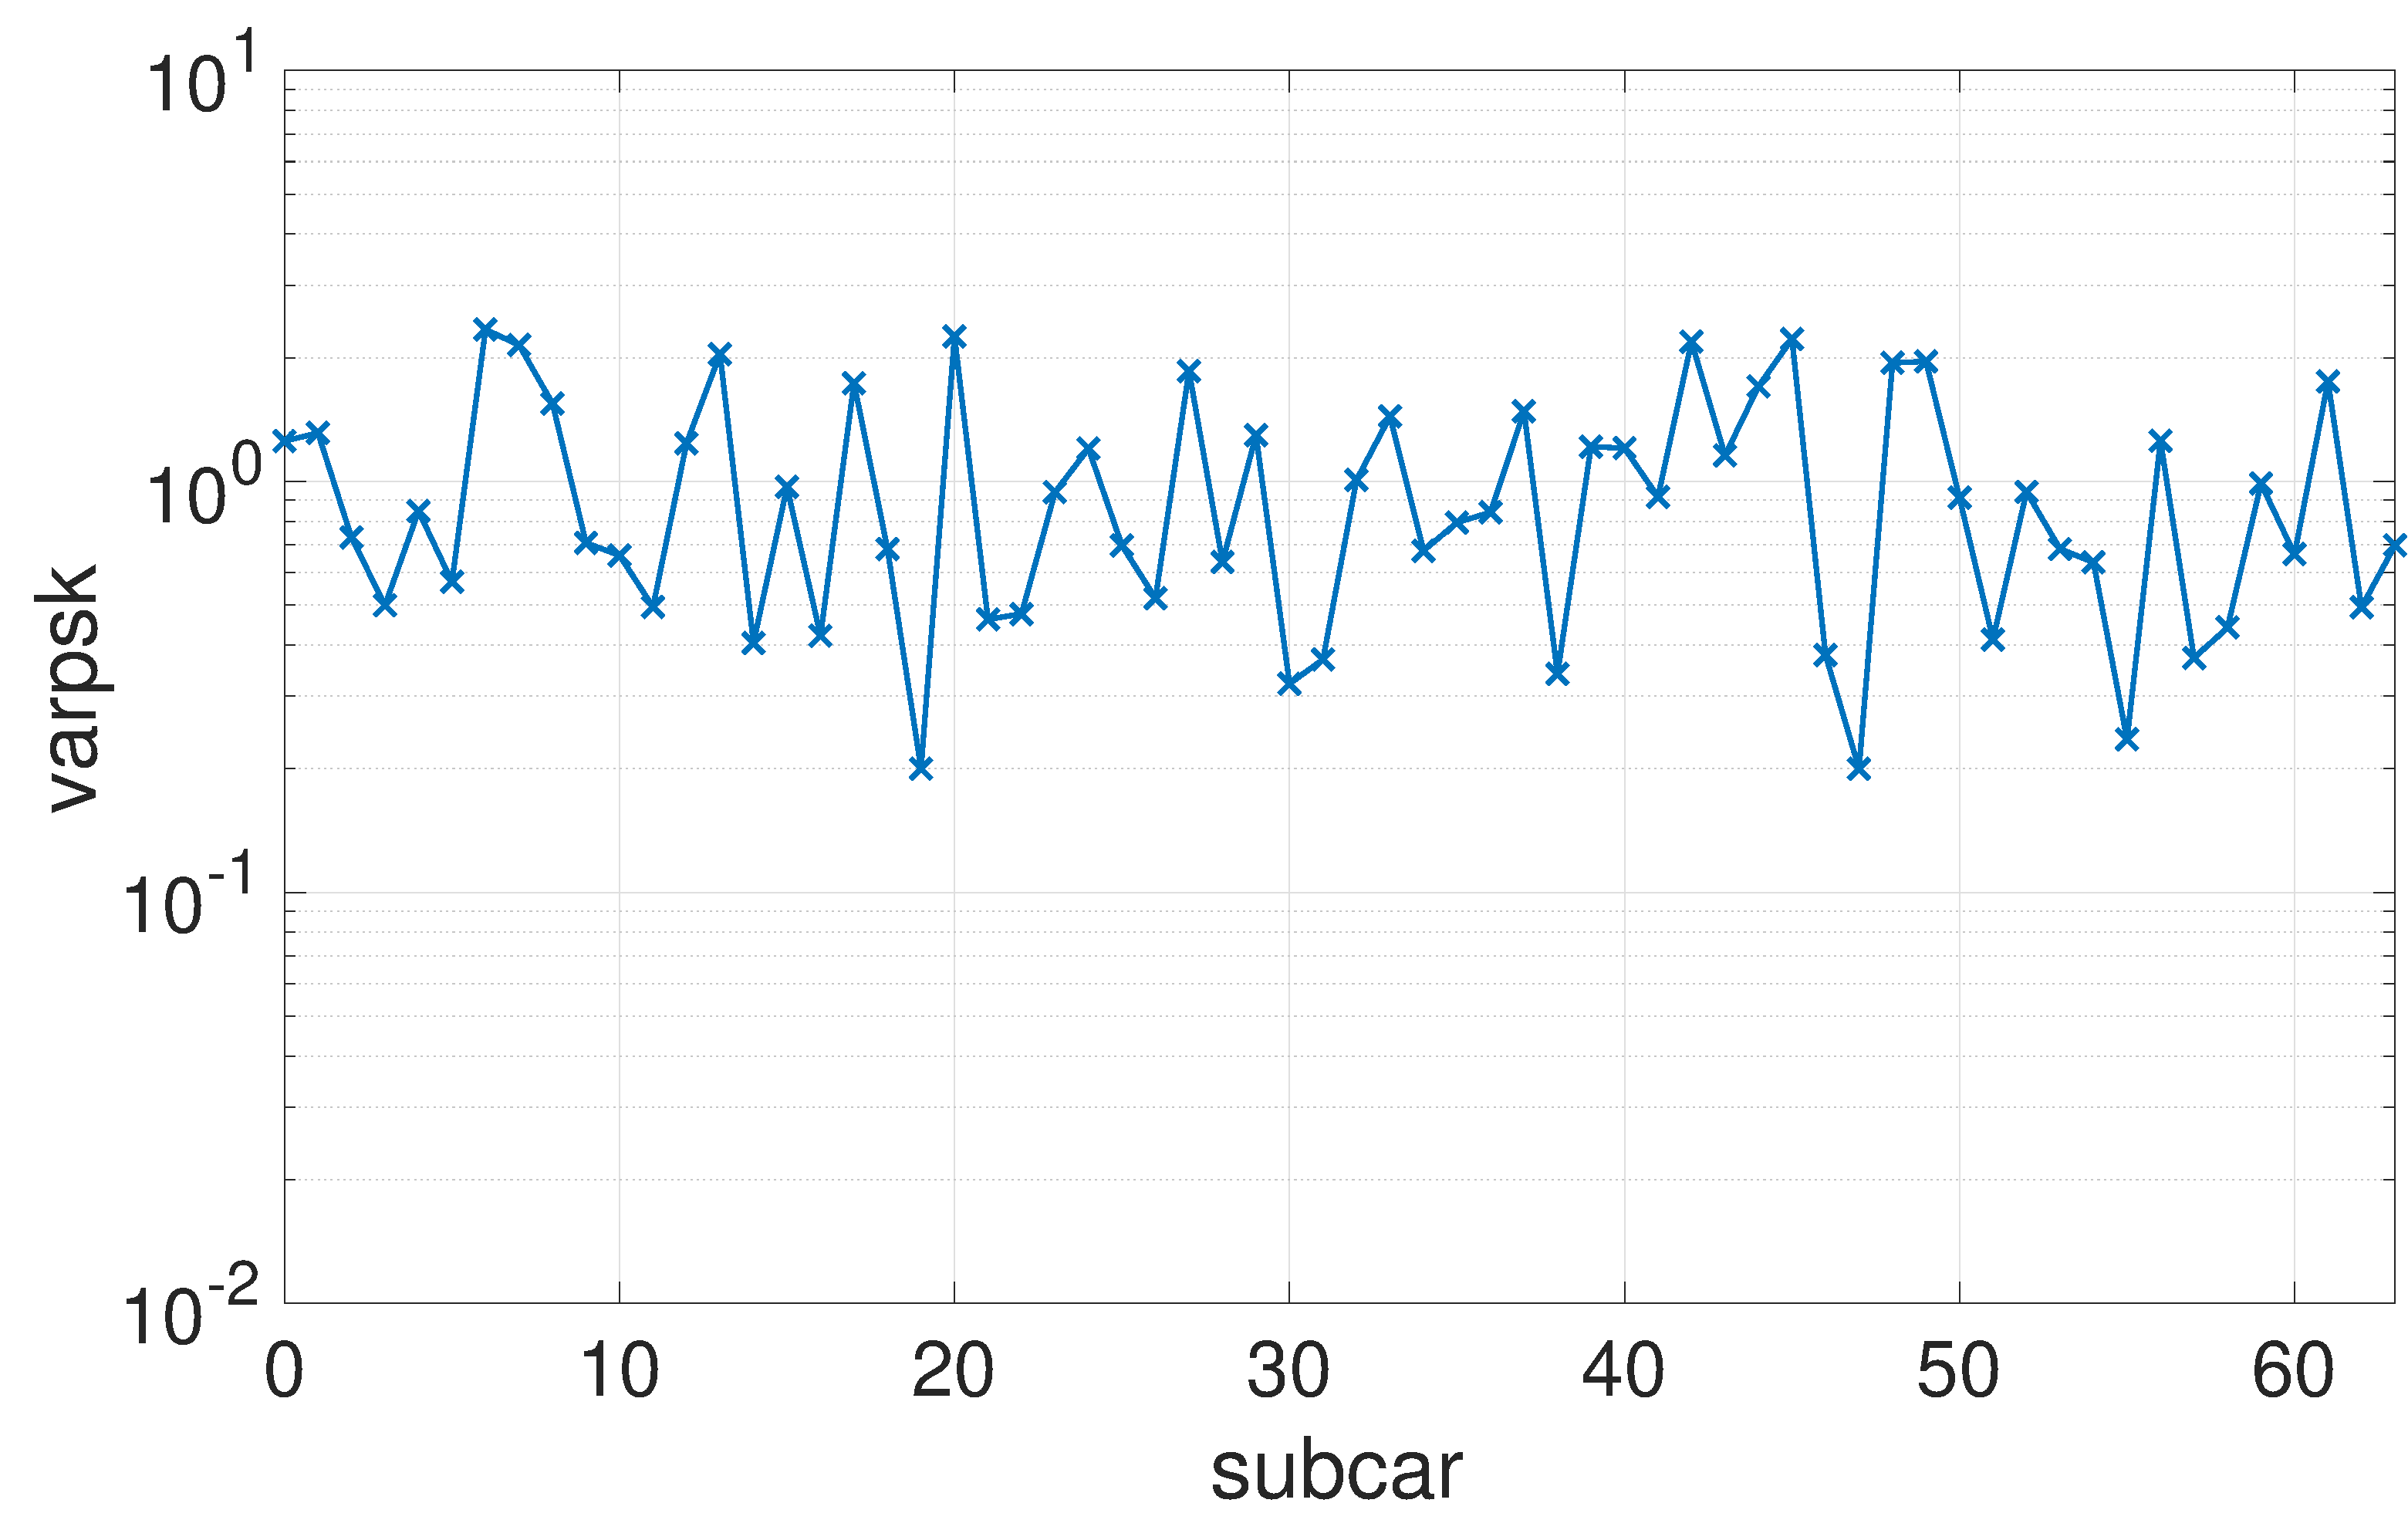
\includegraphics[width=\linewidth]{Figures/varpsk.eps}
\caption{Normalized channel gain profile $\sigma^2_{PS,k}$ between PU TX 
and SU RX.}
\label{fig:2}
\end{figure}

\noindent Moreover, for CA, a rate-matched LDPC encoder is considered. Using the technical specifications in \cite{ETSI2020}, 
a \BGTwo{} parity check matrix is considered with \LiftSize{} and base code rate \(\BaseRate\). 
This code is rate-matched depending on the CA output to give code rates chosen from \(\Omega_{R_c} = \RateSet\). 
The QoS limits are chosen as \(\Mreq = M_{\mathrm{tot}}/3\), \(\Jmax = \JmaxVal\), and \(\preq = \preqVal\). 
Furthermore, Tab.~\ref{tab:ga_params} shows a list of parameters to implement a mixed-integer non-linear optimization problem 
with stochastic chance-based constraints in MATLAB to maximize $\rbSLB$. 
A genetic algorithm (\GA) has been used to exploit its parallel search capability and increase the chance of finding a global optimum to our optimization problem.

\begin{table}[htbp]
\centering
\caption{MATLAB GA parameters for maximization of $\rbSLB$.}
\label{tab:ga_params}
\begin{tabular}{|c|c|} 
\hline
Number of variables & 129 \\
Population size & 500 \\
Max number of generations & 5000 \\
Max number of stall generations & 30 \\
Crossover probability & 0.8 \\
Mutation probability & 0.1 \\
Function tolerance & $1 \times 10^{-6}$ \\
Constraint tolerance & $1 \times 10^{-6}$ \\
Nonlinear constraint solver & penalty \\
Creation function & \texttt{gacreationnonlinearfeasible} \\
\hline
\end{tabular}
\end{table}

For the aforementioned parameters, the CLO performance is
evaluated from the simulated SE values, the optimum code
rates and the number of transmissions required for error-free
transmission as a function of the average energy-per-bit-tonoise
ratio at the SU RX defined by
\begin{equation*}
\eta = \frac{1}{\rbRc \rbsigmaSW^2} \left( \frac{1}{\rbK} \sum_{k \in \rbOmega} \frac{\rbpk \rbsigmaSSk^2}{\rbmk} \right).
\end{equation*}
The CLO is evaluated in the range $\eta \in [0~\text{dB}, \ldots, 40~\text{dB}]$. In Fig.~3, the optimum code rate $\rbRcopt$ selected by the CLO for the cases with and without CC are compared.
\begin{figure}[htbp]
    \centering
    \psfrag{codebest}[c][c]{\scriptsize $\rbRcopt$}
    \psfrag{codenocc}[c][c]{\scriptsize \hspace{2em}$\rbRcopt$-no CC}
    \psfrag{codecc}[c][c]{\scriptsize \hspace{2em}$\rbRcopt$- CC}
    \psfrag{eta}[c][c]{\scriptsize $\rbEtaDB$}
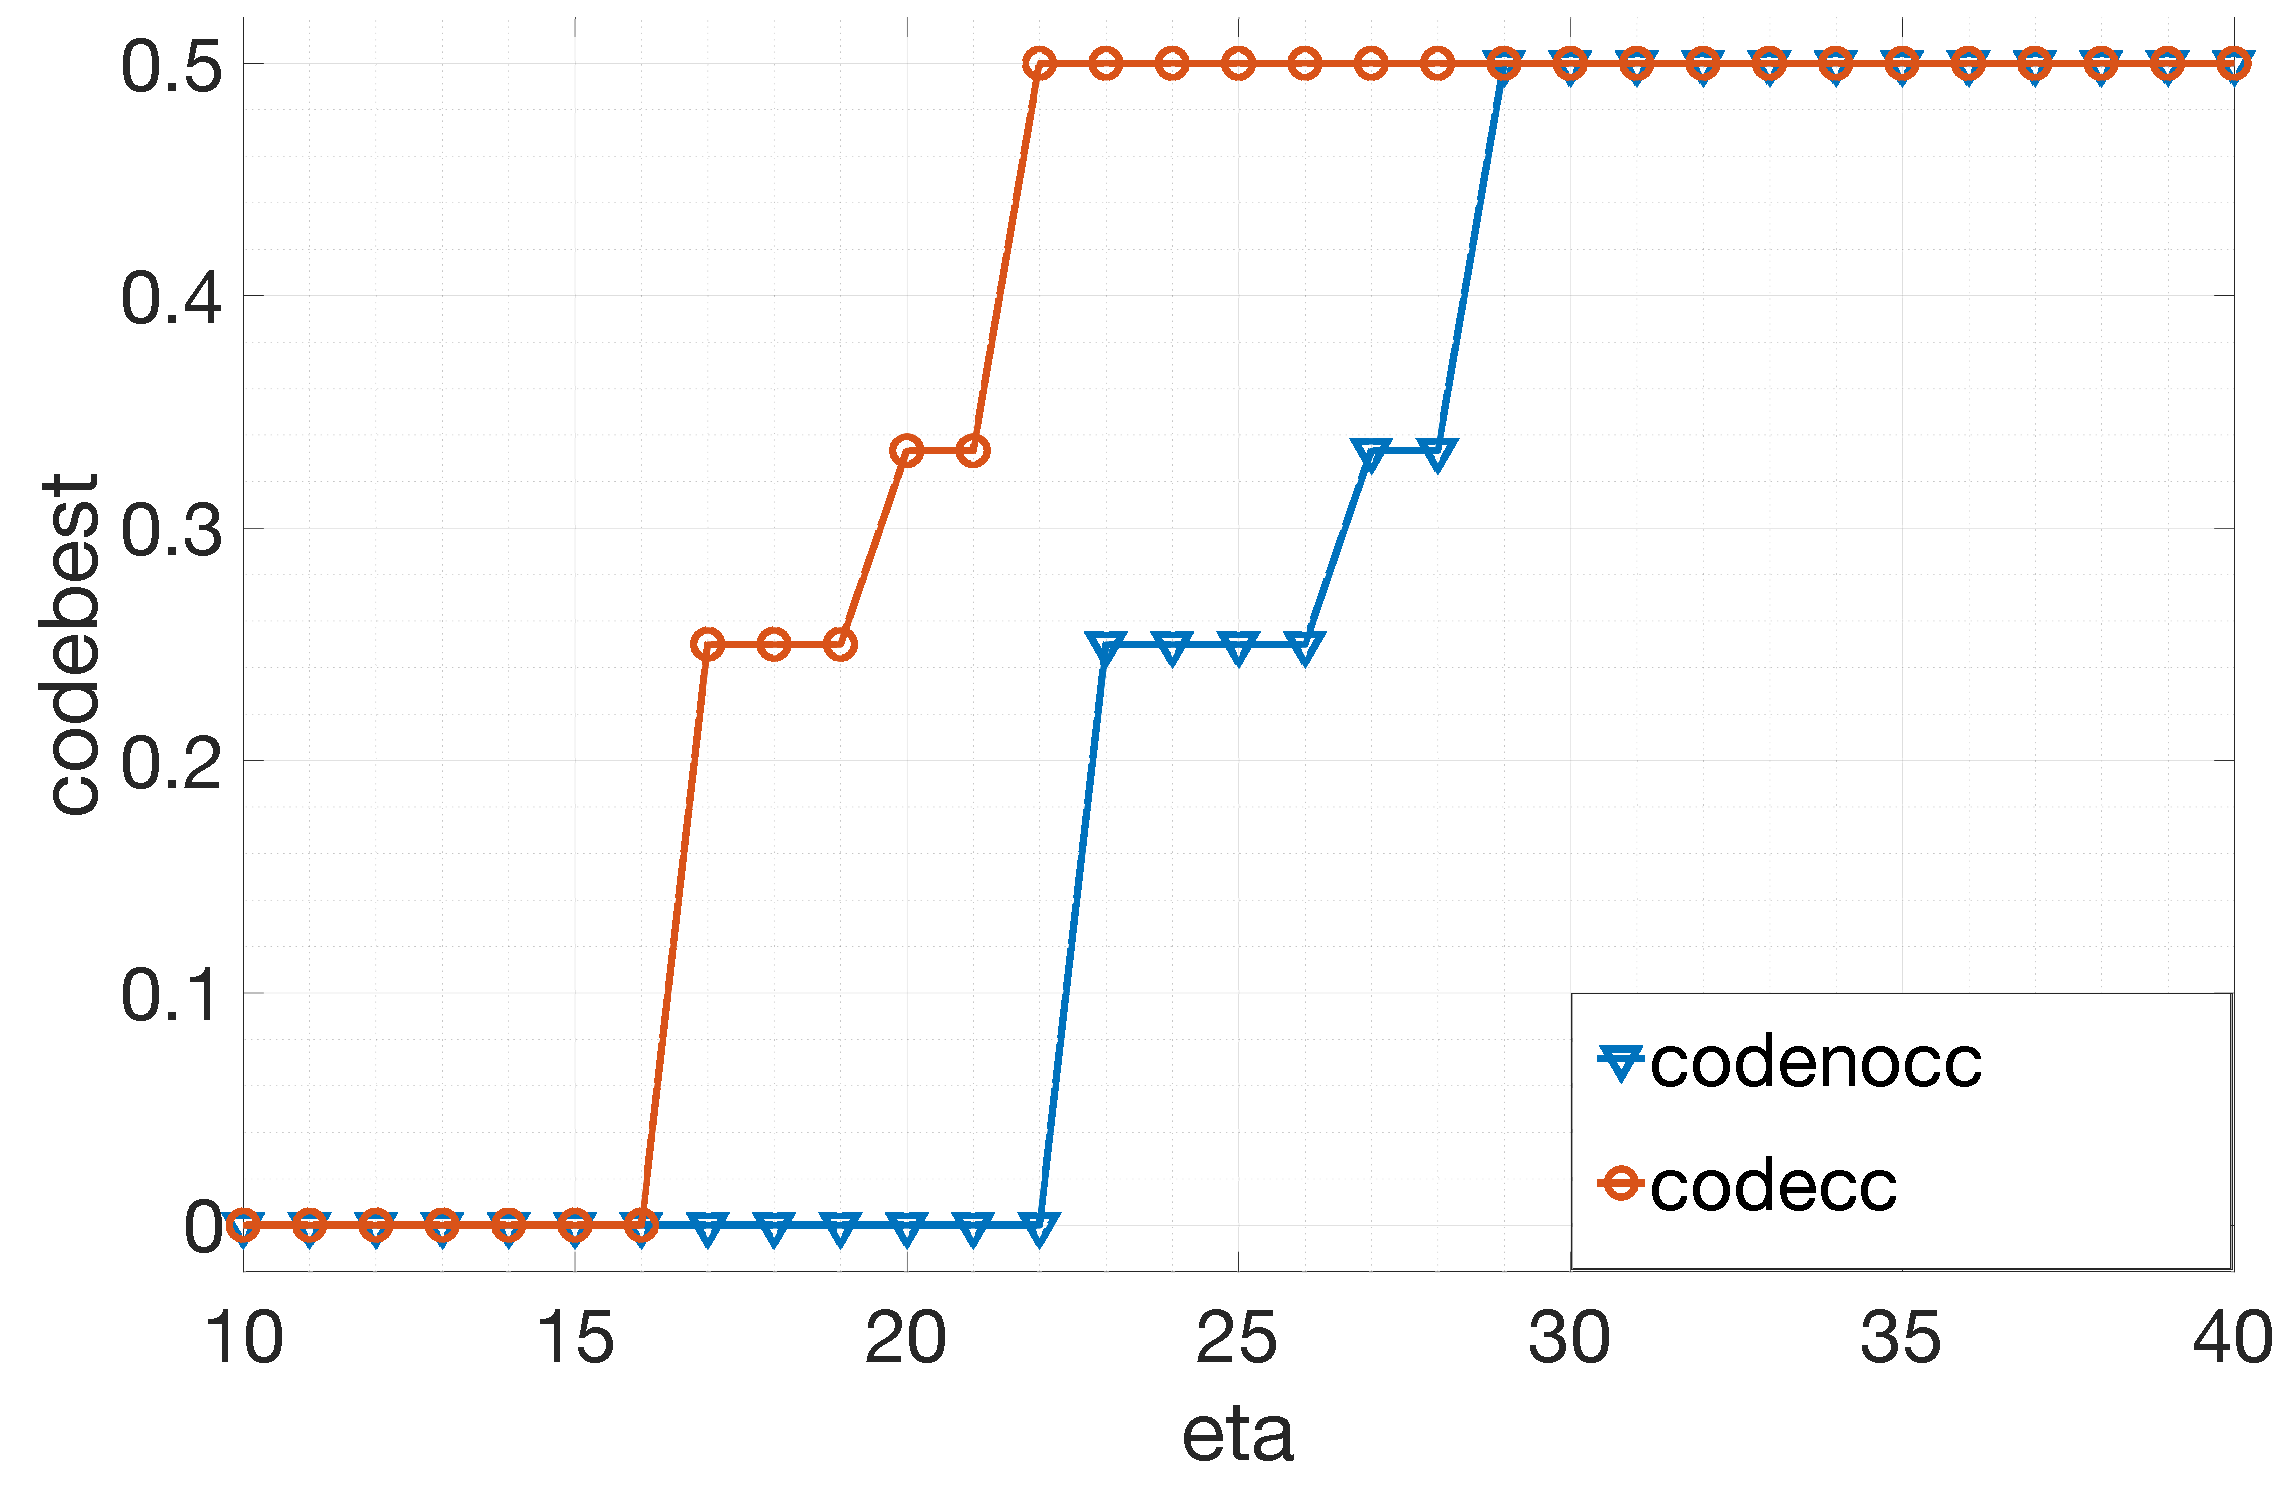
\includegraphics[width=0.8\columnwidth]{Figures/rcscompare_240111.eps}
   \caption{Optimum adaptive coding rate $\hat{R}_{c,\text{opt}}$ versus $\eta$ for $J_{\max} = 2$, $M_{\text{req}} = M_{\text{tot}}/3$, and $p_{\text{req}} = 0.1$.}
    \label{fig:example}
\end{figure}


As can be seen, for the case with (without) CC, the CLO has
no solution up to $17~\text{dB}$ ($23~\text{dB}$), as it, e.g., violates the QoS
constraints in {14} and/or {16}. Clearly, increasing $\eta$ further
allows the CLO to choose higher coding rates from $\rbRc$, where
with CC, one switches to a higher $\rbRcopt$ at smaller $\eta$ compared
to the case without CC.

In Fig.~4, we investigate the gap between the achievable SE $S$
and the lower bound $\rbSLB$ from the CLO for the cases with and
without CC, resp., together with the optimum corresponding
rates $\rbRcopt$ from Fig.~3.

\begin{figure}[htbp]
    \centering
    \psfrag{sslb}[c][c]{\scriptsize $\rbSLB~\rbSLBunit$}         
    \psfrag{slbnocc}[c][c]{\scriptsize\hspace{4em}$\rbSLB~\rbCLOnocc$} 
    \psfrag{slbcc}[c][c]{\scriptsize\hspace{4em} $\rbSLB~\rbCLOcc$} 
    \psfrag{snocc}[c][c]{\scriptsize\hspace{4em} $S~\rbSimnocc$}   
    \psfrag{scc}[c][c]{\scriptsize\hspace{4em} $S~\rbSimcc$} 
    \psfrag{codenocc}[c][c]{\scriptsize \hspace{2em}$\rbRcopt$-no CC}
    \psfrag{codecc}[c][c]{\scriptsize \hspace{2em}$\rbRcopt$- CC}
    \psfrag{eta}[c][c]{\scriptsize $\rbEtaDB$}
    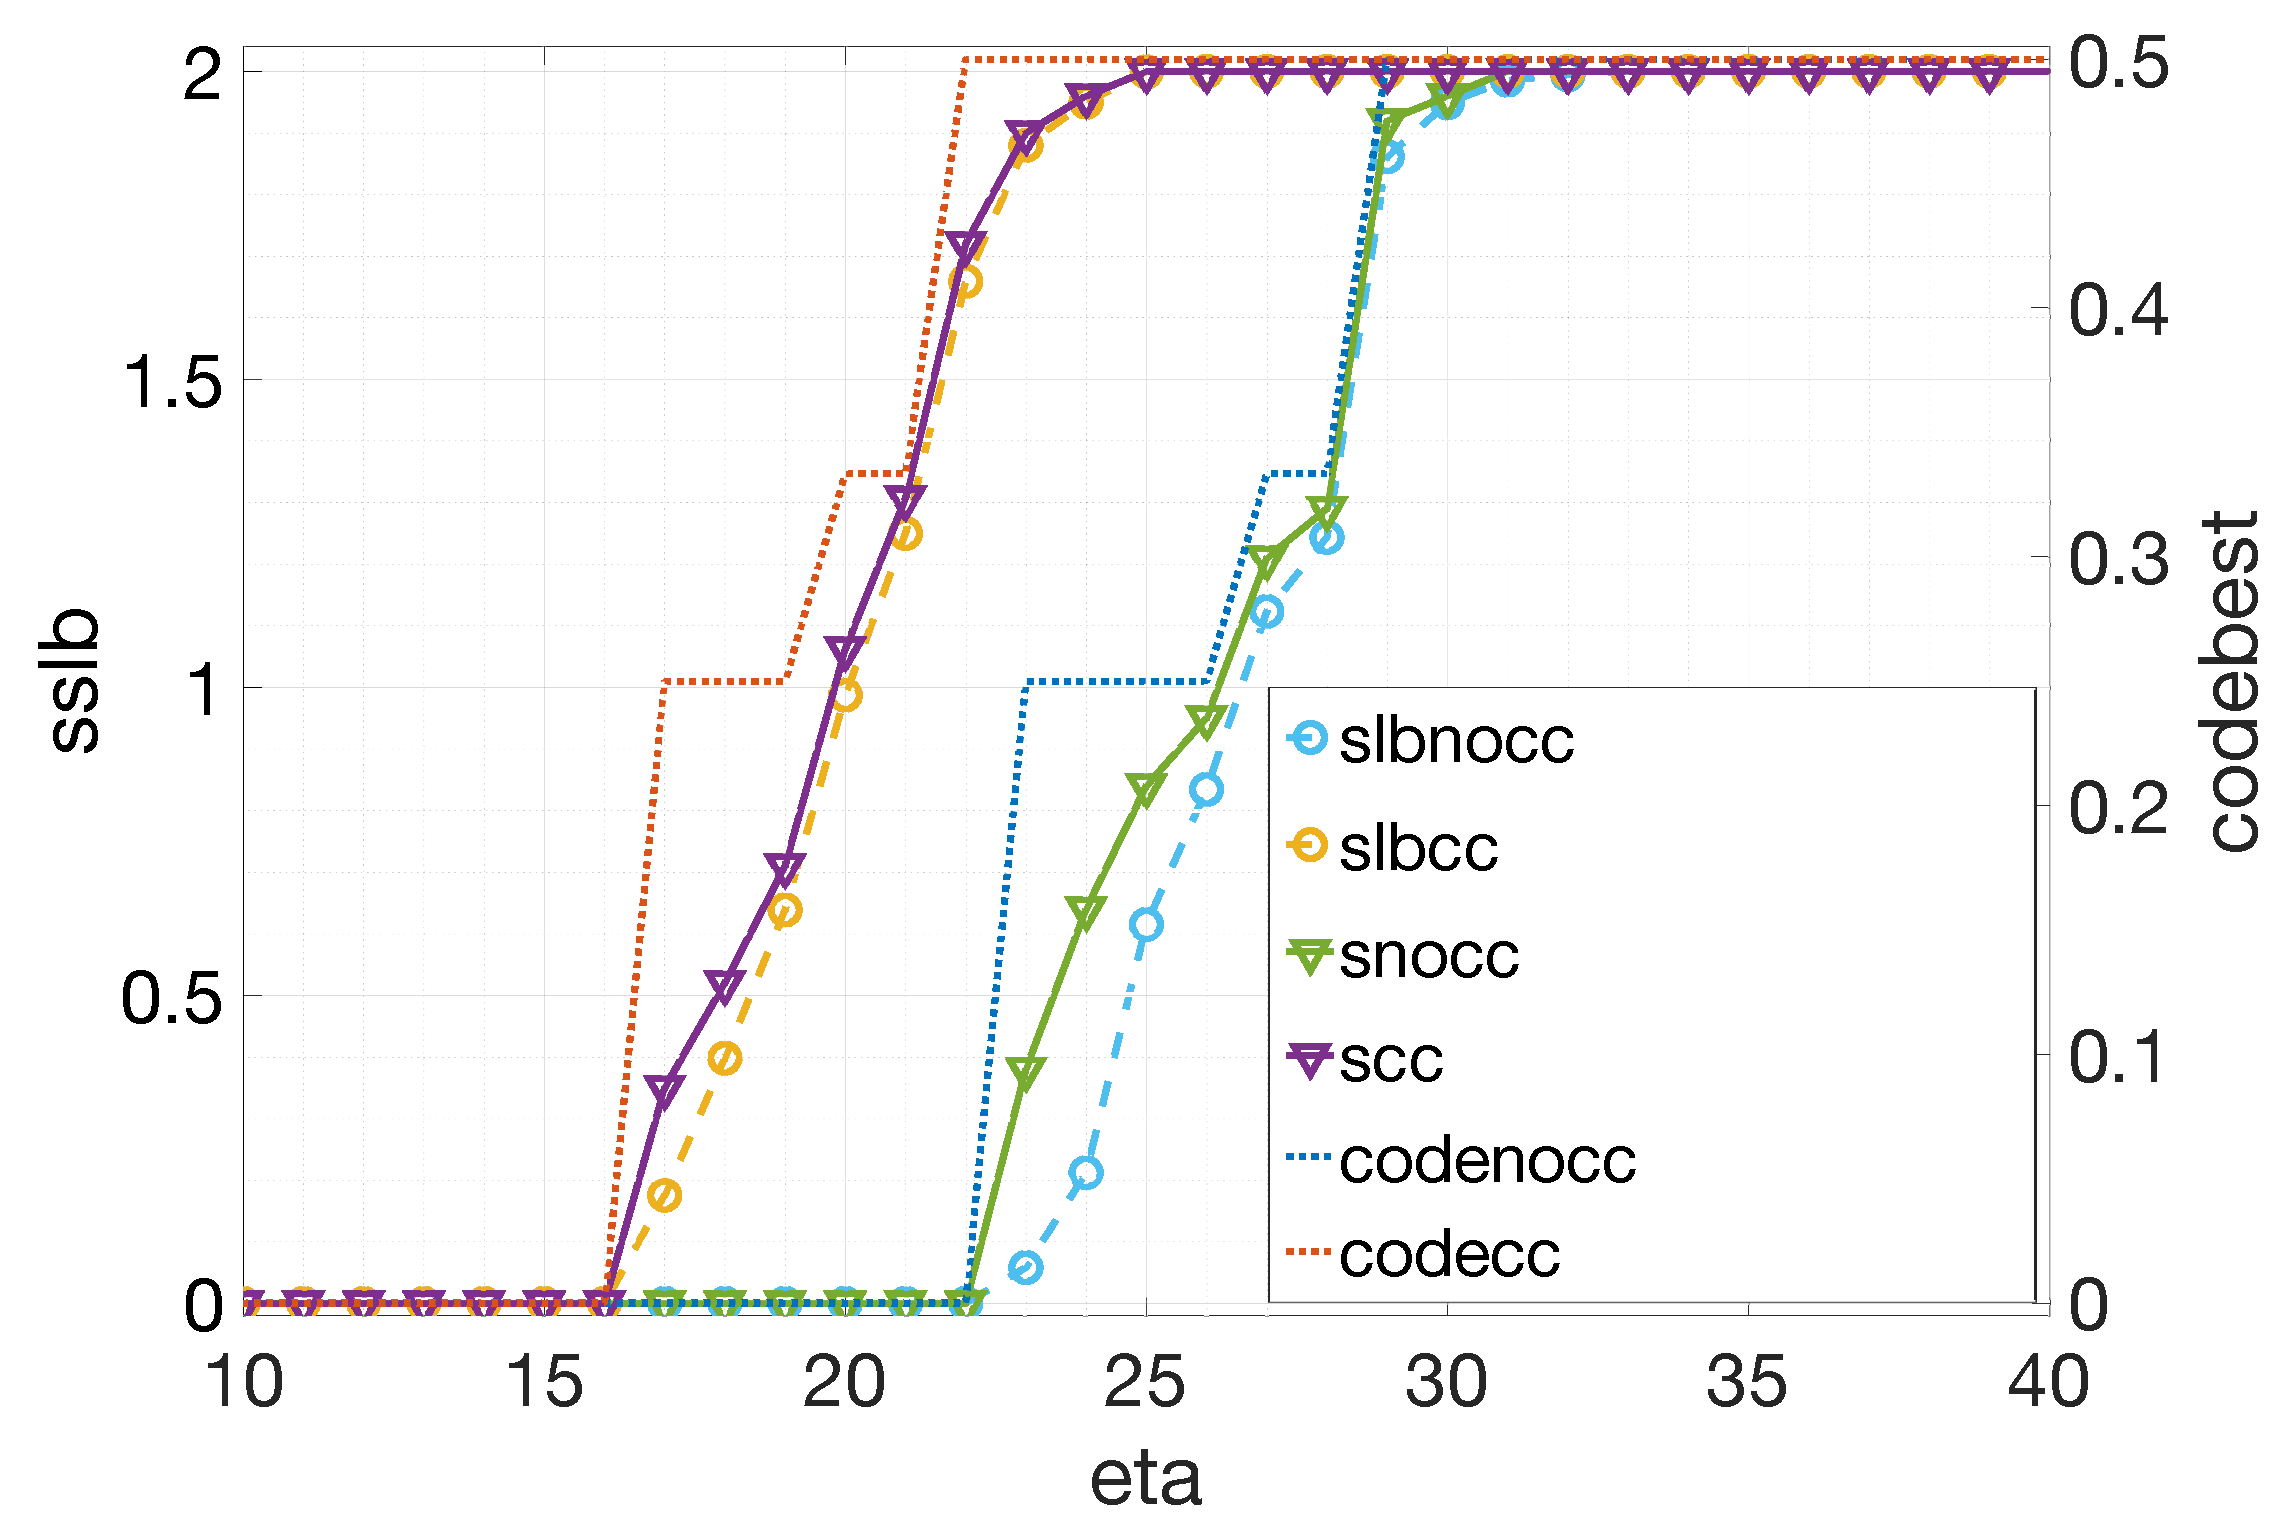
\includegraphics[width=\columnwidth]{Figures/sescompare_240111.eps}
    \caption{Comparison of SE $S$ (solid) and its lower bound 
             $\rbSLB$ (dotted) from CLO versus $\eta$ for $\rbJmax = 2$,
             $\rbMreq = \rbMtot/3$ and $\rbpreq = 0.1$ (left) and corresponding
             optimum rates $\rbRcopt$ (right).} 
    \label{fig:4}
\end{figure}

As the bit-rate constraint in {12} ensures for the chosen $\rbMtot$ 
that we have an average of 4 bits per subcarrier and the 
highest available $\rbRc$ is $\frac{1}{2}$, the maximum achievable SE is 2 
information bits per subcarrier. As seen in Fig.~\ref{fig:4}, $\rbSLB$ lower-bounds
$S$ with the bound tightening as we increase $\eta$. The 
steep changes in SE observed at $\eta \in \{17, 20, 22\}~\text{dB}$ for the 
case with CC and $\eta \in \{23, 27, 29\}~\text{dB}$ for the case without CC,
resp., result from changes in $\rbRcopt$. This change corresponds to 
the optimizer selecting a higher $\rbRcopt$ which maximizes $\rbSLB$. 
As the bit-rate constraint in {12} ensures for the chosen $\rbMtot$ 
that we have an average of 4 bits per subcarrier and the 
highest available $\rbRc$ is $\frac{1}{2}$, the maximum achievable SE is 2 
information bits per subcarrier. As seen in Fig.~\ref{fig:4}, $\rbSLB$ lower-bounds
$S$ with the bound tightening as we increase $\eta$. The 
steep changes in SE observed at $\eta \in \{17, 20, 22\}~\text{dB}$ for the 
case with CC and $\eta \in \{23, 27, 29\}~\text{dB}$ for the case without CC,
resp., result from changes in $\rbRcopt$. This change corresponds to 
the optimizer selecting a higher $\rbRcopt$ which maximizes $\rbSLB$. 
Clearly, in this case, using a CC improves the SE performance 
by approximately $6~\text{dB}$. Finally, in Fig.~\ref{fig:5}, we compare $\bar{J}$ with 
its upper bound $\bar{J}_{\text{UB}}$ from CLO.

\begin{figure}[htbp]
    \centering
\psfrag{nnub}[c][c]{\scriptsize $J,~\rbJUB~\rbJUBunit$} 
\psfrag{nubnocc}[c][c]{\scriptsize \hspace{4em}$\rbJUB~\rbJCLOnocc$} 
\psfrag{nubcc}[c][c]{\scriptsize \hspace{4em}$\rbJUB~\rbJCLOcc$}  
\psfrag{nnocc}[c][c]{\scriptsize \hspace{4em}$\bar{J}~\rbJSimnocc$} 
\psfrag{ncc}[c][c]{\scriptsize \hspace{4em}$\bar{J}~\rbJSimcc$}
    \psfrag{eta}[c][c]{\scriptsize $\rbEtaDB$}
    \psfrag{codenocc}[c][c]{\scriptsize \hspace{2em}$\rbRcopt$-no CC}
    \psfrag{codecc}[c][c]{\scriptsize \hspace{2em}$\rbRcopt$- CC}
    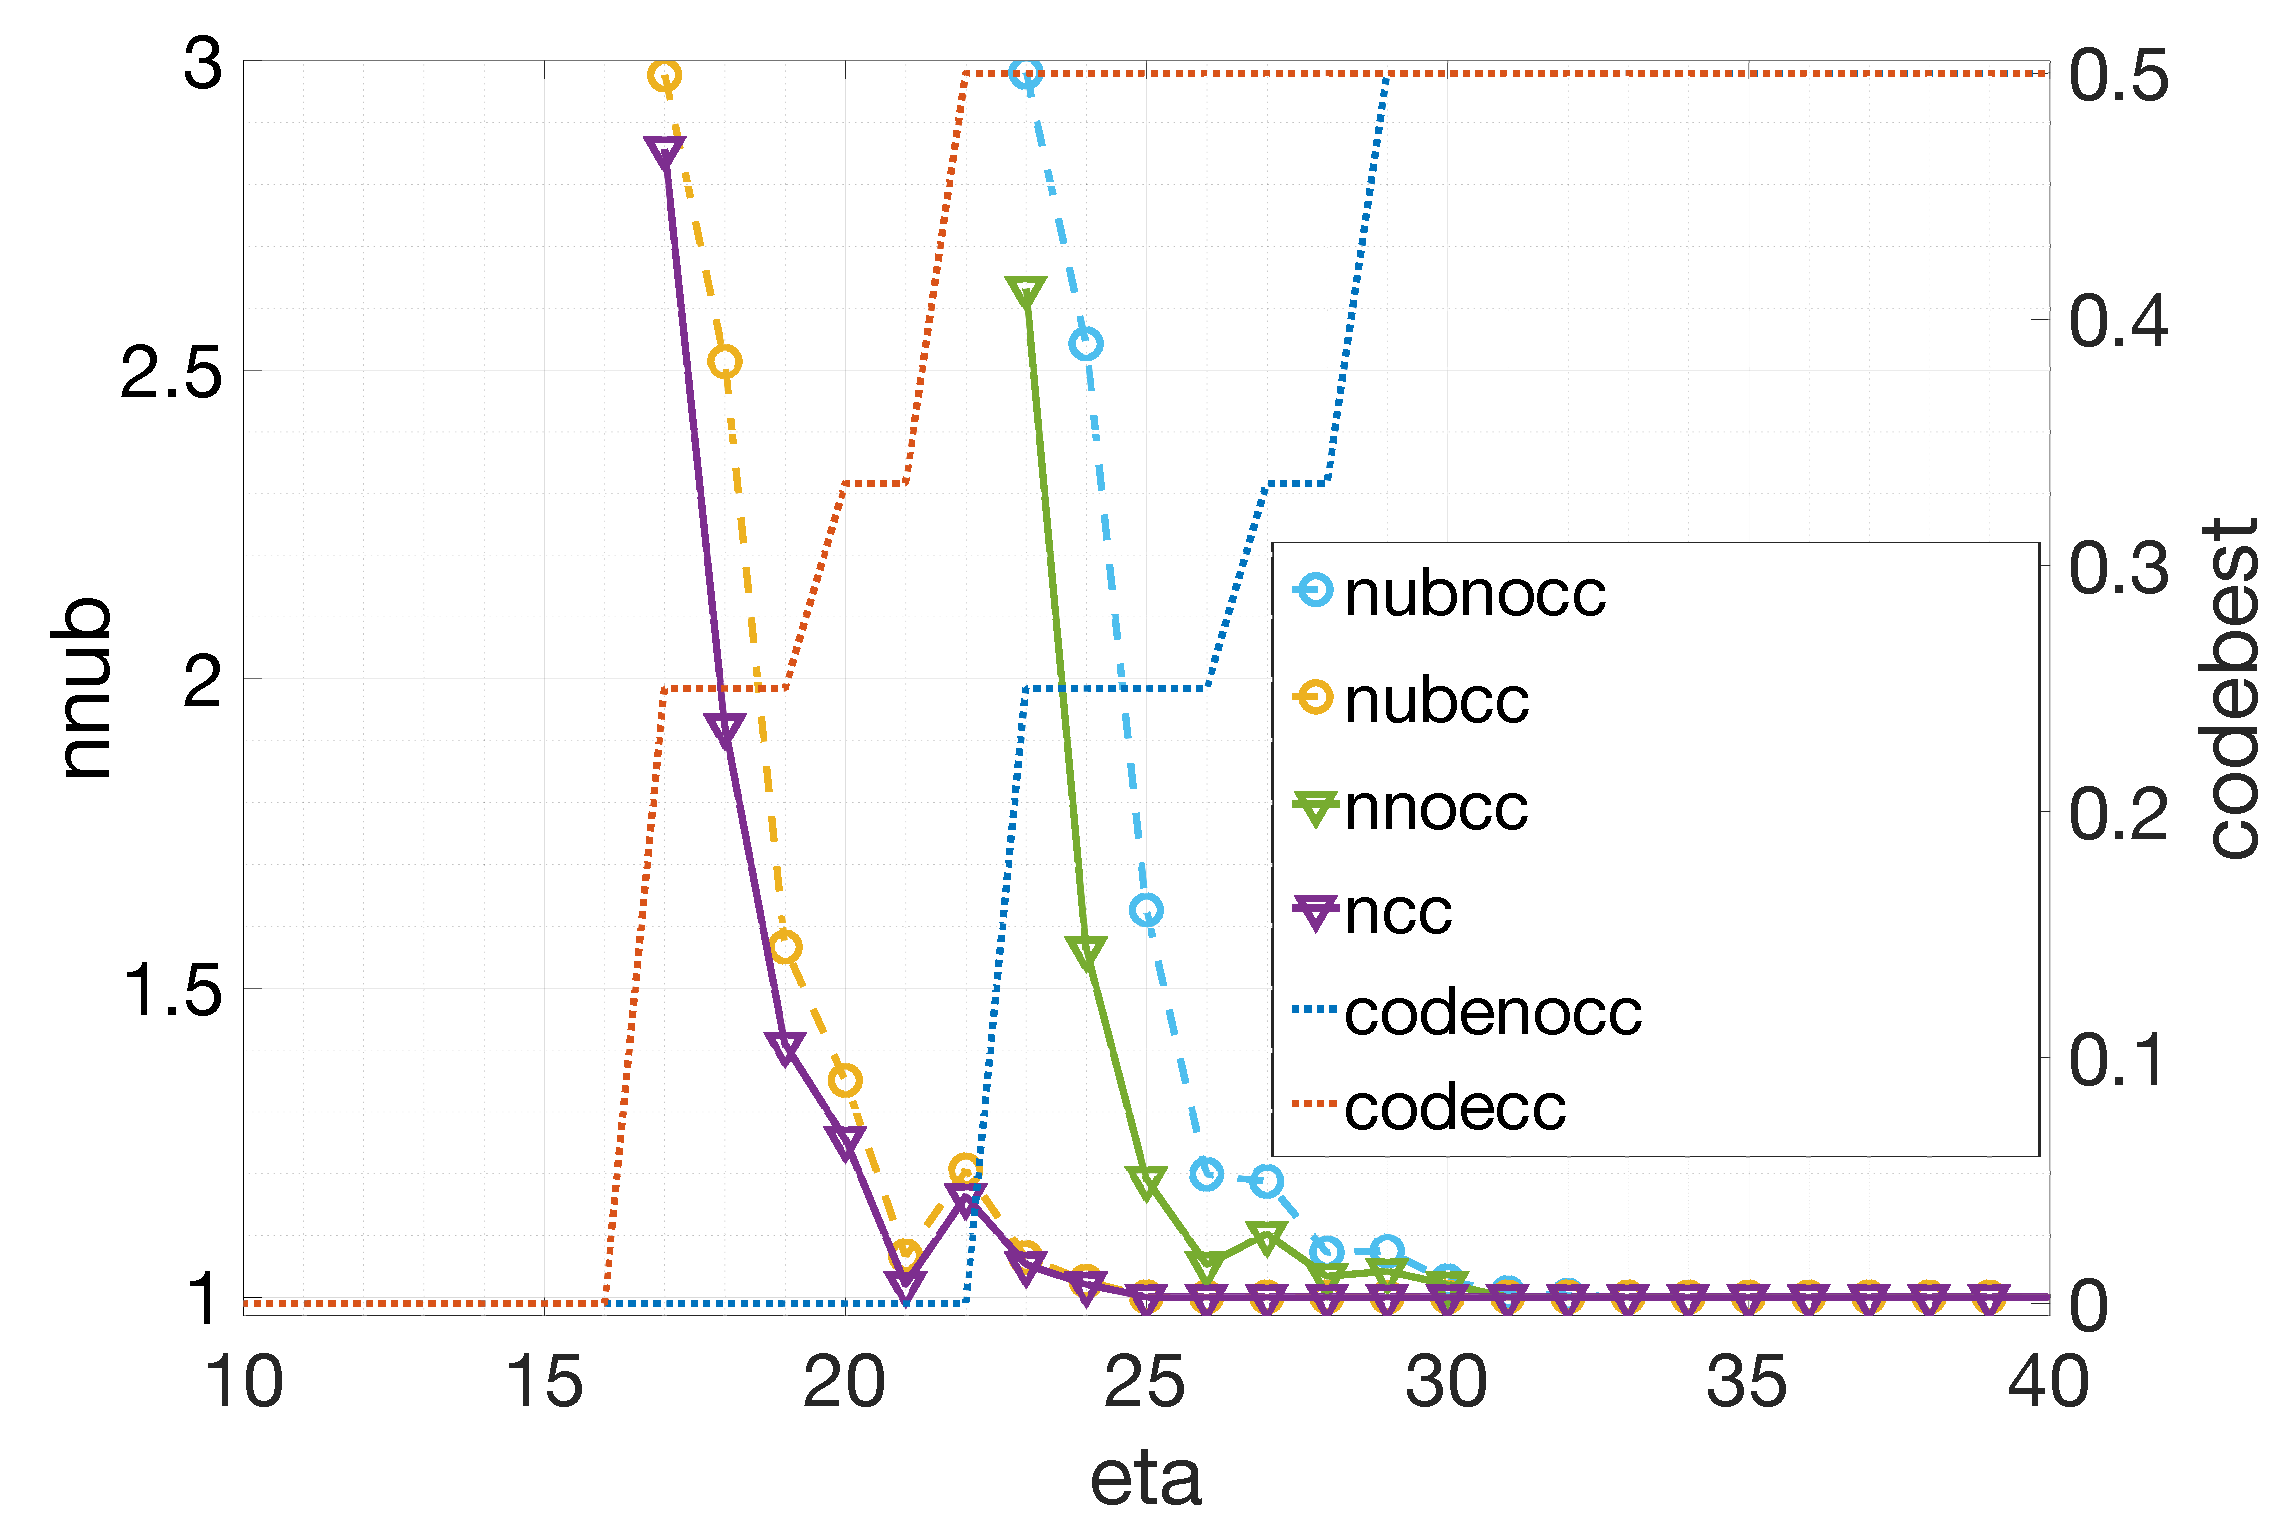
\includegraphics[width=\columnwidth]{Figures/nrscompare_240111.eps} 
    \caption{Comparison of average number $\bar{J}$ (solid) of transmissions
             per packet and its upper bound $\bar{J}_{\text{UB}}$ (dotted)
             from CLO versus $\eta$ for $\rbJmax = 2$, $\rbMreq = \rbMtot/3$
             and $\rbpreq = 0.1$ (left) and corresponding optimum rates
 $\rbRcopt$ (right).}
\label{fig:5}
\end{figure}
As expected, for a certain $\rbRcopt$, at low $\eta$, a large $\bar{J}$ is
observed, which decreases as $\eta$ increases while improving
$S$. The observed steep changes in $\bar{J}$ and $\bar{J}_{\text{UB}}$ correspond to changes of $\rbRcopt$ as discussed for $S$ in Fig.~\ref{fig:4}. Here, although
it leads to an increase in $D$, the optimizer may select an $\rbRcopt$
with higher $\bar{J}_{\text{UB}}$ as the goal is to maximize the $\rbSLB$.
\newpage
changes of $\rbRcopt$ as discussed for $S$ in Fig.~\ref{fig:4}. 
Here, although it leads to an increase in $D$, the optimizer may select 
a $\rbRcopt$ with higher $\bar{J}_{\mathrm{UB}}$ as the goal is to maximize 
$\rbSLB$.
